\chapter{Vortex Pinning}
\label{theoryvortex}

\section{History}
	Superconductivity was first discovered by Heike Kamerlingh Onnes in 1911. He found that by cooling mercury to 4.2 degrees Kelvin, the resistivity of the metal went to 0. This phenomenon has important implications with regards to magnetic fields. One can imagine that as a magnet is placed near a superconductor, Faraday's law will cause a countercurrent to develop inside the superconductor. Due to the lack of resistance, this supercurrent creates a magnetic field that perfectly balances out the input magnetic field, cancelling it out. If the magnetic field is increased, eventually the system reaches a critical current under which the magnetic field can no longer be countered and the superconduction is suppressed. This type of superconductor is referred to as a type I superconductor. There is a second type of superconductor which gets around this problem by allowing some magnetic field to enter in isolated flux lines.

\section{Ginzburg-Landau}
Superconductivity near the transition temperature can be succinctly characterized by a complex order parameter field $\psi$. Near this critical temperature, the free energy of the system becomes
\begin{eqnarray}
F = F_n + \alpha |\psi|^2 + \frac {\beta} {2} |\psi|^4 + \frac {1} {2m} |(-i \hbar \nabla - 2 e \overrightarrow A) \psi|^2 + \frac {|\overrightarrow B |^2} {2 \mu_0}
\label{freeE}
\end{eqnarray}
where $F_n$ is the free energy, $\alpha$ and $\beta$ are system constants which will be defined later,$\mu_0$ is the magnetic permeability of free space , $m$ is the cooper pair effective mass, $e$ is electron charge, $\overrightarrow A$ is the magnetic vector potential, and $\overrightarrow B$ is the magnetic field. Being interested in the physical reprecussions of this kind of system, we minimize the free energy with respect to the order parameter and vector potential to get

\begin{eqnarray}
\alpha \psi + \beta |\psi|^2 \psi \frac {1} {2m} (-i \hbar \nabla - 2 e \overrightarrow A)^2 \psi = 0
\label{GLEQ1}
\end{eqnarray}
\begin{eqnarray}
\nabla \times \overrightarrow B = \mu_0 \overrightarrow j
\label{GLEQ2}
\end{eqnarray}
\begin{eqnarray}
\overrightarrow j = \frac {2e} {m} Re(\psi^* (-i \hbar \nabla - 2 e \overrightarrow A) \psi)
\label{GLEQ3}
\end{eqnarray}
where $j$ is the current and $Re$ is the real part. Equation ~\ref{GLEQ1} can be thought of in two parts. The first part ($\alpha \psi + \beta |\psi|^2 \psi $) is just the component relating to the superconductor, without supercurrent. Above the superconducting temperature, only $\psi = 0$ solves the equation. Below the superconducting temperature we have $|\psi|^2 = -\frac {\alpha} {beta}$, which is reminiscent of a quantum observable. The second half of ~\ref{GLEQ1} is basically a modified version of the Schrodinger time-independent equation, but with a magnetic potential. ~\ref{GLEQ2} is Ampere's law. ~\ref{GLEQ3} is also reminiscent of a quantum observable with $ -i \hbar \nabla - 2e \overrightarrow A$ as the operator. The Ginzburg-Landau equations can be related to the microscopic Bardeen-Cooper-Schrieffer theory ~\cite{Sadovskyy14}. 




\section{Vortices}

\subsection{Vortex-Vortex Interactions}
	This is the type of superconductor we are interested in. Unfortunately, these flux lines will move due to Lorentz forces $W = d \cdot F = d \cdot (B \times I)$ where $W$ is the energy drained away by moving vortices, $d$ is the distance the vortex travels, $F$ is the force on the vortex, $B$ is the field of the vortex, and $I$ is the current of the system. The acceleration of the vortex can be determined using the vortex mass which comes from the Cooper pairs which sustain it. Whether or not a vortex will move is complicated and hard to study analytically. There are many factors which affect the movement of a vortex. First, vortices which rotate in the same direction will push each other away~\ref{sameV}. Conversely, if the vortices spin in the same direction, they will attract and annihilate each other~\ref{diffV}. This can be explained if one looks at the lorentz forces of a vortex-vortex system.

\begin{figure}[htbp]
\begin{center}
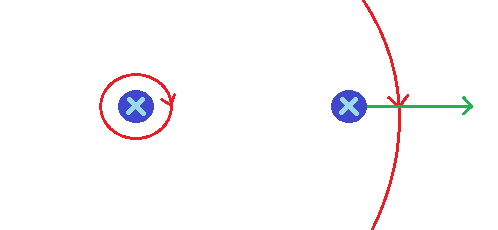
\includegraphics[scale=.50]{sameVortex.png}
\caption{The right hand rule tells us which direction the currents will swirl around a vortex pointing into the page. Then using Lorentz's law  at the second vortex, we can see that the second vortex will be pushed away. The same thing is happening from the current of the second vortex onto the first.}
\label{sameV}
\end{center}
\end{figure}

\begin{figure}[htbp]
\begin{center}
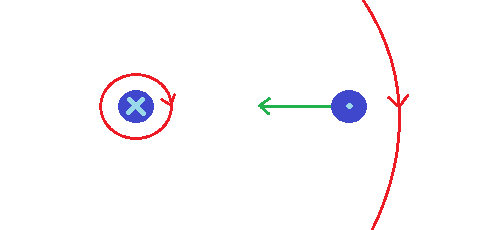
\includegraphics[scale=.50]{oppositeVortex.png}
\caption{The right hand rule tells us which direction the currents will swirl around a vortex pointing into the page. Then using Lorentz's law  at the second vortex, we can see that the second vortex will be pulled in this time. The same thing is happening from the current of the second vortex onto the first (although the second current flows in the opposite direction).}
\label{diffV}
\end{center}
\end{figure}

\subsection{Vortex-Wall Interactions}
The system is not always superconducting. It is also possible to embed non-superconducting components into the system. Since the super-current cannot enter this system (other than evanescently), There are many interesting effects to observe near these zones. First, a vortex near a magnetically neutral non-superconducting zone will be attracted to it. This can be seen as a type of "Venturi effect". Since the current flux must be conserved around a vortex, and there is not as much room for it to flow on the side closest to the wall, the current increases. A difference in current flux on opposing sides of the vortex then creates a force in the direction of the wall. The vortex is then pulled into the wall. The vortex will tend to remain there until pushed out by an external force. Two of the most common forces are external applied current and other vortices.
 
